\documentclass[9pt]{beamer}
\renewcommand\textbullet{\ensuremath{\bullet}}

\usepackage{sty/opencg3-spec}
\usepackage{sty/opencg3-spec-beamer}
\usepackage{xspace,bookmark,lmodern,mathtools,color,multido,ulem,upquote,tabularx}
\usepackage[T1]{fontenc}
\usefonttheme[onlymath]{serif}
\setcounter{tocdepth}{4}

\newcommand{\Version}[0]{Version 0.2.10}
\newcommand{\PrjName}{OpenCG\texorpdfstring{\textsuperscript{3}}}
\newcommand{\PrjNameFull}{Open Command-oriented\\Geometric Graphics Generator}
\newcommand{\PrjSpec}{\PrjName{} Specification \Version}

\title[\PrjSpec]{\PrjNameFull}
\subtitle{\small \PrjSpec}


\author[KVD \and ADL]{Dong Nai-Jia \inst{1} \and Lin Yong-Hsiang \inst{2}}
\institute{	\inst{1} National Chiao Tung University\\Department of Computer Science \and
			\inst{2} National Taiwan University\\Department of Agricultural Chemistry}
\date[\today]{\today}


\begin{document}
\beamertemplatenavigationsymbolsempty

\section{OpenGC3}

\begin{frame}
	\titlepage
\end{frame}


\section{Overview}

\subsection{Definition}

\subsubsection{Token}

\begin{frame}[t] \frametitle{Command Tokens}

	\begin{block}{Regular Expressions}
		$\MSN \coloneqq \{\ \alpha \mid \alpha \in \texttt{[0-9]+} \ \}$ \\ [.24em]
		$\MSR \coloneqq \{\ \alpha \mid \alpha \in \texttt{[+\textbackslash-]?([0-9]*[.])?[0-9]+}\ \}$ \hfill
		$\Rightarrow \MSR \supset \MSN \ $ \\ [.24em]
		$\MSS \coloneqq \{\ \alpha \mid \alpha \in \texttt{\SingleQuote(.*?)\SingleQuote|[.0-9A-Za-z+\textbackslash-]+} \ \}$ \hfill
		$\Rightarrow \MSS \supset \MSR \ $ \\ [.24em]
		$\MSW \coloneqq \{\ \alpha \mid \alpha \in \texttt{[ \textbackslash{}t]} \}$ \hfill whitespace
	\end{block}

	\begin{block}{Descriptions}
		\begin{itemize}
			\item The matching mechanism abides by the maximal munch rule.
			\item Each command is whitespace-insensitive except being quoted by a pair of single quotation marks (\SingleQuote).
		\end{itemize}
	\end{block}

\end{frame}

\subsubsection{Grammar}

\begin{frame}[t] \frametitle{Command Grammars}

	\begin{block}{Context-Free Expansions}
		$\left.\CMD \EXP \ARG \CMD \SEP \,\text{;}\, \SEP \,\texttt{EOL} \right.$ \\ [.24em]
		$\left.\ARG \EXP \TUP(\ARG) \SEP \VCT(\ARG) \SEP \SET(\ARG) \SEP
		 \LST(\ARG) \SEP \LST(\ARG, \ARG, \cdots, \ARG) \SEP \MSN \SEP \MSR \SEP \MSS \right.$ \\ [.27em]
		$\left.\text{%
		\begin{tabular}{@{}l}%
			$\TUP(\Pi) \EQV \Tup{\Pi}{n} \EXP \texttt{\TupBrkL}     \ \, \Sigma(\Pi, n) \ \, \texttt{\TupBrkR}$ \\ [.24em]
			$\VCT(\Pi) \EQV \Vct{\Pi}{n} \EXP \texttt{\VctBrkTextL} \ \, \Sigma(\Pi, n) \ \, \texttt{\VctBrkTextR}$ \\ [.24em]
			$\SET(\Pi) \EQV \Set{\Pi}{n} \EXP \texttt{\SetBrkL}     \ \, \Sigma(\Pi, n) \ \, \texttt{\SetBrkR}$
		\end{tabular}} \right\|\kern.128em$%
		\begin{tabular}{@{}l}%
			$\ \Sigma(\Pi, n) \EXP \overbrace{\Pi \ \cdots \ \Pi}^{n \ \text{items}} \quad\,\ \text{(identical)}$ \\ [.43em]
			$\ \LST(\Pi) \EQV \Lst{\Pi}{n} \EXP \texttt{\LstBrkL} \ \, \Sigma(\Pi, n) \ \, \texttt{\LstBrkR}$
		\end{tabular} \\ [.24em]
		$\left.\LST(\Pi_1,\Pi_2,\cdots,\Pi_{n-1},\Pi_n) \EQV \LstFull{\Pi_1\,\Pi_2\cdots\Pi_{n-1}\,\Pi_n} \EXP
		 \texttt{\LstBrkL} \ \, \Pi_1\cdots\Pi_n \ \, \texttt{\LstBrkR}\right.$
	\end{block}

	\begin{block}{Descriptions}
		\begin{itemize}
			\item Each command starts from $\CMD$ and ends with a \texttt{;} or an \texttt{EOL}.
			\item Non-terminal symbol expansions are prior than function expansions except that symbols are used for describing arguments of a command.
		\end{itemize}
	\end{block}

\end{frame}

\subsubsection{Syntax}

\begin{frame}[t] \frametitle{Command Parsing}

	\begin{block}{Escape Sequence}
		\begin{itemize}
			\item \texttt{\textbackslash x} is an escape sequence.
			\item If \texttt{x} is \texttt{\textbackslash}, then it is treated as a single backslash.
			\item If \texttt{x} is \texttt{EOL} which may vary from platforms, then the sequence is omitted.
			\item Otherwise, the sequence is ignored and triggers a warning by default.
		\end{itemize}
	\end{block}

	\begin{block}{Error Handling}
		\begin{itemize}
			\item Physical lines are separated by an \texttt{EOL}.
			\item Logical lines are separated by either a semicolon or an unescaped \texttt{EOL}.
			\item If the command cannot be parsed by the grammar, then all the characters on the same logical line will be discarded.
		\end{itemize}
	\end{block}

\end{frame}

\subsubsection{System}

\begin{frame}[t] \frametitle{System Hierarchy}

	\begin{block}{Classes}
		\begin{itemize}
			\item Classes are split into two categories, top and bottom.
			\item Top classes are class window, class camera, and data classes.
			\item Bottom classes are class attrib and class group.
			\item Data classes are split into primitive classes and compound classes.
			\item Primitive classes are class point, etc.
			\item Compound classes are class line, class polygon, etc.
		\end{itemize}
	\end{block}

	\begin{block}{Objects}
		\begin{itemize}
			\item An object is instantiated from a class aforementioned.
			\item An object has an unique name throughout the category of its class.
		\end{itemize}
	\end{block}

	\begin{block}{Relations}
		\begin{itemize}
			\item References are bidirectional and can be created or deleted via commands.
		\end{itemize}
	\end{block}

\end{frame}

\subsection{Projection}

\subsubsection{Perspective}

\begin{frame} \frametitle{Perspective Projection}

	\begin{figure}[t]
		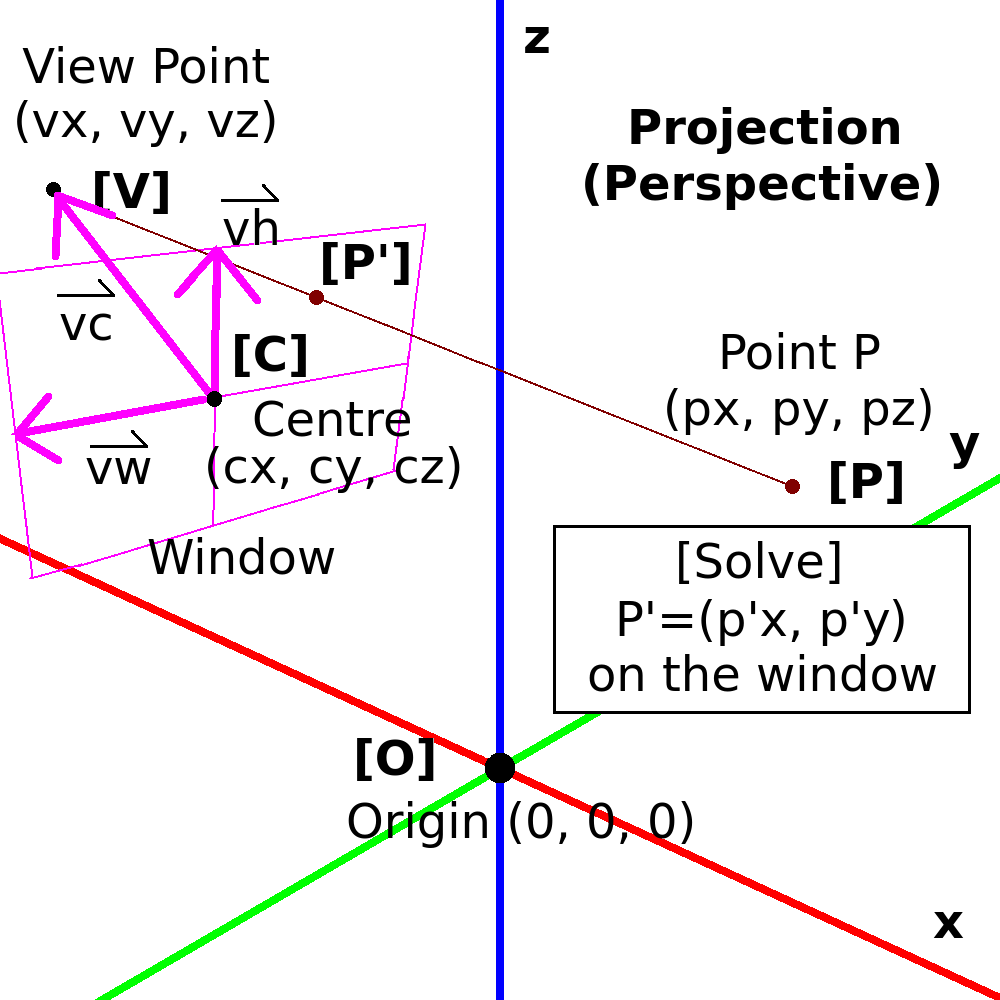
\includegraphics[width=.5\columnwidth]{fig/perspective-projection.png}
		\caption{Projection in Euclidean $\mathbb{R}^3$ Space}
	\end{figure}

\end{frame}


\section{Command}

\subsection{Window}

\subsubsection{Create}

\begin{frame}[t] \frametitle{Create a Window}

	\begin{block}{Command} \newcolumntype{R}{>{\raggedleft\arraybackslash}X}
		\begin{tabularx}{\textwidth}{@{}l@{}l@{}R}
			\InstrName{create window} &
				\ParamMust{\StrName{\Label{w}}} & \InstrItem
		\end{tabularx}
	\end{block}

	\begin{block}{Parametres} \begin{itemize}
		\ParamItem{\Label{w}} the name of the object instantiated from the class window
	\end{itemize} \end{block}

	\begin{block}{Examples}
		\CommandEx{create window main}
	\end{block}

\end{frame}

\subsubsection{Delete}

\begin{frame}[t] \frametitle{Delete a Window}

	\begin{block}{Command} \newcolumntype{R}{>{\raggedleft\arraybackslash}X}
		\begin{tabularx}{\textwidth}{@{}l@{}l@{}l@{}R}
			\InstrName{delete window} &
				\ParamMust{\StrName{\Label{w}}} &
			  	\ParamOptl{\StrName{string}} & \InstrItem
		\end{tabularx}
	\end{block}

	\begin{block}{Parametres} \begin{itemize}
		\ParamItem{\Label{w}} the name of the object instantiated from the class window
		\ParamItem{string}    the text printed right after exiting the session
	\end{itemize} \end{block}

	\begin{block}{Examples}
		\CommandEx{delete window main}
		\CommandEx{delete window main \SingleQuote Have a nice day.\SingleQuote}
	\end{block}

\end{frame}

\subsection{Camera}

\subsubsection{Create}

\begin{frame}[t] \frametitle{Create a Camera}

	\begin{block}{Command} \newcolumntype{R}{>{\raggedleft\arraybackslash}X}
		\begin{tabularx}{\textwidth}{@{}l@{}l@{}l@{}l@{}l@{}R}
			\InstrName{create camera} &
				\ParamMust{\StrName{\Label{c}}} &
				\ParamMust{\TupName{\MSR}{3}{centre}} &
				\ParamMust{\TupName{\Vct{\MSR}{3}}{2}{plane}} &
				\ParamMust{\VctName{\MSR}{3}{sight}} & \InstrItem
		\end{tabularx}
	\end{block}

	\begin{block}{Parametres} \begin{itemize}
		\ParamItem{\Label{c}} the name of the object instantiated from the class camera
		\ParamItem{centre}    the world coordinate $(c_x, c_y, c_z)$ of the centre of the viewport
		\ParamItem{plane}     the horizontal and the vertical vertors $(\vec{v_w}, \vec{v_h})$ of the viewport
		\ParamItem{sight}     the reverse line of sight $\vec{v_c}$ from \Param{centre} to the camera
	\end{itemize} \end{block}

	\begin{block}{Examples}
		\CommandEx{create camera z-top \TupText{0 0 1} \TupText{\VctText{1 0 0} \VctText{0 1 0}} \VctText{0 0 1}}
	\end{block}

\end{frame}

\subsubsection{Select}

\begin{frame}[t] \frametitle{Select a Camera}

	\begin{block}{Command} \newcolumntype{R}{>{\raggedleft\arraybackslash}X}
		\begin{tabularx}{\textwidth}{@{}l@{}l@{}l@{}R}
			\InstrName{select camera} &
				\ParamMust{\StrName{\Label{c}}} &
				\ParamMust{\StrName{\Label{w}}} & \InstrItem
		\end{tabularx}
	\end{block}

	\begin{block}{Parametres} \begin{itemize}
		\ParamItem{\Label{c}} the name of the object instantiated from the class camera
		\ParamItem{\Label{w}} the name of the object instantiated from the class window
	\end{itemize} \end{block}

	\begin{block}{Examples}
		\CommandEx{select camera z-top main}
	\end{block}

\end{frame}

\subsection{Point}

\subsubsection{Create}

\begin{frame}[t] \frametitle{Create Points}

	\begin{block}{Command} \newcolumntype{R}{>{\raggedleft\arraybackslash}X}
		\begin{tabularx}{\textwidth}{@{}l@{}l@{}l@{}R}
			\InstrName{create point } &
			  	\ParamMust{\SetOptl{\StrName{\Label{p}}}{}} &
			  	\ParamMust{\TupName{\MSR}{3}{coord}} & \InstrItem \\
			\InstrName{create point } &
				\ParamMust{\Tup{\StrName{\Label{p}}}{\,\geqslant n}} &
				\ParamMust{\Tup{\TupName{\MSR}{3}{coord}}{n}} & \InstrItem
		\end{tabularx}
	\end{block}

	\begin{block}{Parametres} \begin{itemize}
		\ParamItem{\Label{p}} the name of the object instantiated from the class point
		\ParamItem{coord}     the world coordinate $(p_x, p_y, p_z)$ of the object named \Param{\Label{p}}
	\end{itemize} \end{block}

	\begin{block}{Examples}
		\CommandEx{create point \SingleQuote origin\SingleQuote \ \ \ \TupText{0 0 0}}
		\CommandEx{create point \SetText{X-1 X-2} \ \TupText{1 0 0}}
		\CommandEx{create point \TupText{Y-1 Z-1} \TupText{\TupText{0 1 0}\TupText{0 0 1}}}
	\end{block}

\end{frame}

\subsubsection{Delete}

\begin{frame}[t] \frametitle{Delete Points}

	\begin{block}{Command} \newcolumntype{R}{>{\raggedleft\arraybackslash}X}
		\begin{tabularx}{\textwidth}{@{}l@{}l@{}R}
			\InstrName{delete point } &
				\ParamMust{\SetOptl{\StrName{\Label{p}}}{}} & \InstrItem
		\end{tabularx}
	\end{block}

	\begin{block}{Parametres} \begin{itemize}
		\ParamItem{\Label{p}} the name of the object instantiated from the class point
	\end{itemize} \end{block}

	\begin{block}{Examples}
		\CommandEx{delete point \ origin}
		\CommandEx{delete point \SetText{origin \SingleQuote random-point\SingleQuote}}
	\end{block}

\end{frame}

\subsection{Attribute}

\subsubsection{Create}

\begin{frame}[t] \frametitle{Create Attributes}

	\begin{block}{Command} \newcolumntype{R}{>{\raggedleft\arraybackslash}X}
		\begin{tabularx}{\textwidth}{@{}l@{}l@{}l@{}R}
			\InstrName{create attrib} &
				\ParamMust{\SetOptl{\StrName{attrib}}{}} &
				\ParamMust{\LstOptl{\LstFull{\StrName{\Class{t}} \ \LstOptl{\StrName{prop} \ \ArgName{value}}{}}}{}} & \InstrItem \\
			\InstrName{create attrib} &
				\ParamMust{\Tup{\StrName{attrib}}{}} &
				\ParamMust{\Lst{\LstFull{\StrName{\Class{t}} \ \LstOptl{\StrName{prop} \ \ArgName{value}}{}}}{}} & \InstrItem
		\end{tabularx}
	\end{block}

	\begin{block}{Parametres} \begin{itemize}
		\ParamItem{attrib}    the name of the object instantiated from the class attrib
		\ParamItem{\Class{t}} the name of one of the top classes
		\ParamItem{prop}      the property of the object of \Param{\Class{t}}
		\ParamItem{value}     the value of \Param{prop} in designated format
	\end{itemize} \end{block}

	\begin{block}{Examples}
		\CommandEx{create attrib \TupText{magenta dashed-and-translucent-line} \EOLText
		                         \LstText{\LstText{point fill-hsv \TupText{300 1.0 1.0}} \EOLText
		                       \ \LstText{line \LstText{style dashed} \LstText{fill-rbga \LstText{\TupText{0 255 0} 0.5}}}}}
	\end{block}

\end{frame}

\subsubsection{Attach}

\begin{frame}[t] \frametitle{Attach Attributes}

	\begin{block}{Command} \newcolumntype{R}{>{\raggedleft\arraybackslash}X}
		\begin{tabularx}{\textwidth}{@{}l@{}l@{}l@{}R}
			\InstrName{attach attrib} &
				\ParamMust{\TupOptl{\StrName{attrib}}{}} &
				\ParamMust{\SetOptl{\StrName{label}}{}} & \InstrItem \\
			\InstrName{attach attrib} &
				\ParamMust{\Tup{\StrName{attrib}}{}} &
				\ParamMust{\Tup{\StrName{label}}{}} & \InstrItem
		\end{tabularx}
	\end{block}

	\begin{block}{Parametres} \begin{itemize}
		\ParamItem{attrib}    the name of the object instantiated from the class attrib
		\ParamItem{label}     the name of the object instantiated from one of the top classes
	\end{itemize} \end{block}

	\begin{block}{Examples}
		\CommandEx{attach attrib \ red \quad \quad \quad \ \ point-0}
		\CommandEx{attach attrib \TupText{red large} \ point-1}
		\CommandEx{attach attrib \ blue \quad \quad \quad \SetText{point-2 rect-0}}
		\CommandEx{attach attrib \TupText{5px black} \SetText{point-3 circ-0}}
		\CommandEx{attach attrib \TupText{red thick} \TupText{point-4 line-0 triangle-0}}
	\end{block}

\end{frame}

\subsection{Operation}

\subsubsection{Assign}

\begin{frame}[t] \frametitle{Assign Operations}

	\begin{block}{Command} \newcolumntype{R}{>{\raggedleft\arraybackslash}X}
		\begin{tabularx}{\textwidth}{@{}l@{}l@{}l@{}l@{}R}
			\InstrName{assign operat} &
				\ParamMust{\StrName{action}} &
				\ParamMust{\StrName{class}} &
				\ParamOptl{\MSNName{repeat}\ \ValueDefn{=\infty}} & \InstrItem
		\end{tabularx}
	\end{block}

	\begin{block}{Parametres} \begin{itemize}
		\ParamItem{action}    the name of the corresponding action of \Param{class}
		\ParamItem{class}     the name of one of the classes
		\ParamItem{repeat}    the amount of the commands emitting operation names
	\end{itemize} \end{block}

	\begin{block}{Examples}
		\CommandEx{assign operat create point 2}
		\CommandEx{x-axis \TupText{1 0 0}}
		\CommandEx{y-axis \TupText{0 1 0}}
		\CommandEx{// Back To Normal}
	\end{block}

\end{frame}


\end{document}

